
\label{matrix}
\begin{center}
\RRR{20}
\end{center}

\begin{tabular}{|c|c|} \hline  
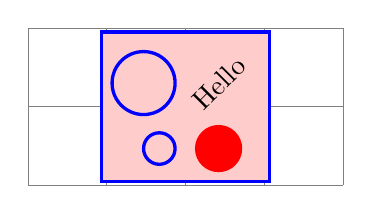
\begin{tikzpicture}[baseline=1cm]
\draw[help lines] (0,0) grid (4,2);
\node [matrix,fill=red!20,draw=blue,very thick] (my matrix) at (2,1)
{
\draw (0,0) circle (4mm); & \node[rotate=45] {Hello}; \\
\draw (0.2,0) circle (2mm); & \fill[red] (0,0) circle (3mm); \\
};
\end{tikzpicture}
& 
\parbox{10cm}{
\BS{node} [\RDD{matrix},fill=red!10,draw=blue,very thick] at (2,1) \\
\{ \\
\BS{draw} (0,0) circle (4mm); \& \BS{node} [rotate=45] {Hello}; \BS{}\BS{} \\
\BS{draw}  (0.2,0) circle (2mm); \& \BS{fill}[red] (0,0) circle (3mm); \BS{}\BS{} \\
\}; \\
}
\\ \hline 
\end{tabular} 

\bigskip

\begin{tabular}{|c|c|} \hline  
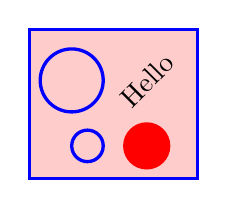
\begin{tikzpicture}[baseline=0pt]
\matrix [fill=red!20,draw=blue,very thick] 
{
\draw (0,0) circle (4mm); & \node[rotate=45] {Hello}; \\
\draw (0.2,0) circle (2mm); & \fill[red] (0,0) circle (3mm); \\
};
\end{tikzpicture}
&  
\parbox{10cm}{
\BSS{matrix} [fill=red!10,draw=blue,very thick] \\
\{ \\
\BS{draw} (0,0) circle (4mm); \& \BS{node} [rotate=45] {Hello}; \BS{}\BS{} \\
\BS{draw}  (0.2,0) circle (2mm); \& \BS{fill}[red] (0,0) circle (3mm); \BS{}\BS{} \\
\}; \\
}
\\ \hline 
\end{tabular} 


\SbSbSSCT{Alignement des cellules}{Cell Pictures}


\begin{center}
\RRR{20-3}
\end{center}

\begin{tabular}{|c|c|c|} \hline  
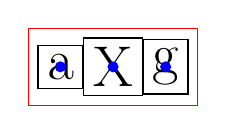
\begin{tikzpicture}
[every node/.style={draw=black,font=\huge}]
\matrix [draw=red]
{
\node {a}; \fill[blue] (0,0) circle (2pt); &
\node {X}; \fill[blue] (0,0) circle (2pt); &
\node {g}; \fill[blue] (0,0) circle (2pt); \\
};
\end{tikzpicture}
&  
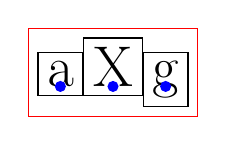
\begin{tikzpicture}
[every node/.style={draw=black,anchor=base,font=\huge}]
\matrix [draw=red]
{
\node {a}; \fill[blue] (0,0) circle (2pt); &
\node {X}; \fill[blue] (0,0) circle (2pt); &
\node {g}; \fill[blue] (0,0) circle (2pt); \\
};
\end{tikzpicture}
&  
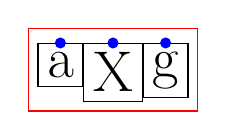
\begin{tikzpicture}[every node/.style={draw=black}]
\matrix [draw=red,anchor=north,font=\huge]
{
\node {a}; \fill[blue] (0,0) circle (2pt); &
\node {X}; \fill[blue] (0,0) circle (2pt); &
\node {g}; \fill[blue] (0,0) circle (2pt); \\
};
\end{tikzpicture}
\\ \hline  
 & anchor=base &  anchor=north \\ \hline 
\end{tabular} 

\bigskip
\begin{tabular}{|c|c|c|} \hline  
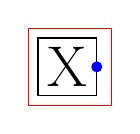
\begin{tikzpicture}
[every node/.style={draw=black,font=\huge}]
\matrix [draw=red]
{

\node[left]  {X}; \fill[blue] (0,0) circle (2pt);  \\
};
\end{tikzpicture}
&  
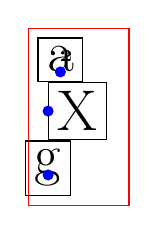
\begin{tikzpicture}
[every node/.style={draw=black,anchor=base,font=\huge}]
\matrix [draw=red]
{
\node {a}; \fill[blue] (0,0) circle (2pt); ²\\
\node[right] {X}; \fill[blue] (0,0) circle (2pt);  \\
\node {g}; \fill[blue] (0,0) circle (2pt); \\
};
\end{tikzpicture}
&  
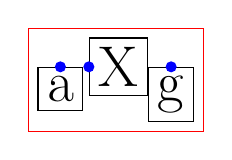
\begin{tikzpicture}[every node/.style={draw=black}]
\matrix [draw=red,anchor=north,font=\huge]
{
\node {a}; \fill[blue] (0,0) circle (2pt); &
\node[right] {X}; \fill[blue] (0,0) circle (2pt); &
\node {g}; \fill[blue] (0,0) circle (2pt); \\
};
\end{tikzpicture}
\\ \hline  
 & anchor=base &  anchor=north \\ \hline 
\end{tabular} 

\bigskip

\begin{tabular}{|c|c|} \hline  
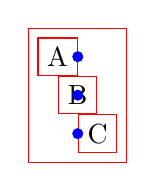
\begin{tikzpicture}[baseline=0pt]
\matrix [draw=red,nodes=draw]
{
\node[left] {A}; \fill[blue] (0,0) circle (2pt); \\
\node {B}; \fill[blue] (0,0) circle (2pt); \\
\node[right] {C}; \fill[blue] (0,0) circle (2pt); \\
};
\end{tikzpicture}
&  
\parbox{12cm}{
\BS{matrix} [draw=red,nodes=draw]
\AC{\\
\BS{node}\rouge{[left]} {A}; \BS{fill}[blue] (0,0) circle (2pt); \BS{} \BS{} \\
\BS{node} {B}; \BS{fill}[blue] (0,0) circle (2pt);\BS{} \BS{} \\
\BS{node}\rouge{[right]} {C}; \BS{fill}[blue] (0,0) circle (2pt); \BS{} \BS{}\\
}; \\
}

\\ \hline 
\end{tabular} 

\bigskip

\begin{tabular}{|c|c|} \hline  
\multicolumn{2}{|c|}{\BS{matrix} [draw,\RDD{column  sep}=1cm,nodes=draw]} 
\\ \hline 
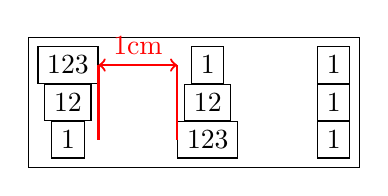
\begin{tikzpicture}
\matrix [draw,column sep=1cm,nodes=draw]
{
\node(a) {123}; & \node (b) {1}; & \node {1}; \\
\node {12}; & \node {12}; & \node {1}; \\
\node(c) {1}; & \node (d) {123}; & \node {1}; \\
};
\draw [red,thick] (a.east) -- (a.east |- c)
(d.west) -- (d.west |- b);
\draw [<->,red,thick] (a.east) -- (d.west |- b)
node [above,midway] {1cm};
\end{tikzpicture}
&  
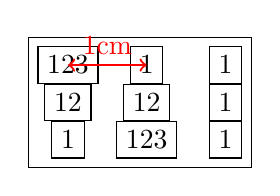
\begin{tikzpicture}
\matrix [draw,column sep={1cm,between origins},nodes=draw]
{
\node(a) {123}; & \node (b) {1}; & \node {1}; \\
\node {12}; & \node {12}; & \node {1}; \\
\node {1}; & \node {123}; & \node {1}; \\
};
\draw [<->,red,thick] (a.center) -- (b.center) node [above,midway] {1cm};
\end{tikzpicture}
\\ \hline \RDD{column sep}=1cm & column sep=\AC{1cm,\RDD{between origins} } 
\\ \hline 
\end{tabular} 

\bigskip

\begin{tabular}{|c|c|} \hline
\multicolumn{2}{|c|}{\BS{matrix} [draw,\RDD{row sep}=1cm,nodes=draw]} 
\\ \hline 
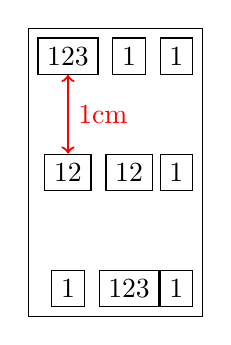
\begin{tikzpicture}
\matrix [draw,row sep=1cm,nodes=draw]
{
\node (a) {123}; & \node {1}; & \node {1}; \\
\node (b) {12}; & \node {12}; & \node {1}; \\
\node {1}; & \node {123}; & \node {1}; \\
};
\draw [<->,red,thick] (a.south) -- (b.north) node [right,midway] {1cm};
\end{tikzpicture}
&
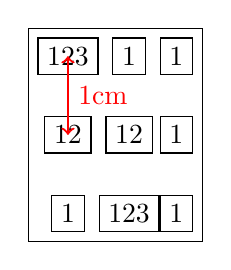
\begin{tikzpicture}
\matrix [draw,row sep={1cm,between origins},nodes=draw]
{
\node (a) {123}; & \node {1}; & \node {1}; \\
\node (b) {12}; & \node {12}; & \node {1}; \\
\node {1}; & \node {123}; & \node {1}; \\
};
\draw [<->,red,thick] (a.center) -- (b.center) node [right,midway] {1cm};
\end{tikzpicture}
\\  \hline 
\RDD{row sep}=1cm  & row sep=\AC{1cm,\RDD{between origins} } 
\\ \hline 


\end{tabular} 




\bigskip

\begin{tabular}{|c|c|} \hline  
\multicolumn{2}{|c|}{\BS{matrix} [ \rouge{row sep=5mm},draw,nodes=draw]} \\
\multicolumn{2}{|c|}{ \{ \BS{node} \AC{1}; \& \BS{node} \AC{2}; \& \BS{node} \AC{3}; \BS{}\BS{}  } \\
\multicolumn{2}{|c|}{ \BS{node} \AC{4} ; \& \BS{node}  \AC{5}; \& \BS{node}  \AC{6};  \BS{}\BS{} \rouge{[1cm]} } \\
\multicolumn{2}{|c|}{ \BS{node} \AC{7}; \& \BS{node}\AC{8}; \& \BS{node}\AC{9}; \BS{}\BS{} \}  } 
\\ \hline  
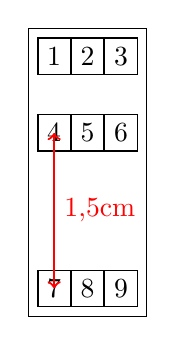
\begin{tikzpicture}
\matrix [row sep=5mm,draw,nodes=draw]
{
\node {1}; & \node {2};& \node {3}; \\
\node(a) {4} ; & \node {5}; & \node {6};\\[1cm]
\node(b) {7}; &\node {8}; & \node {9}; \\
};
\draw [<->,red,thick] (a.center) -- (b.center) node [right,midway] {1,5cm};
\end{tikzpicture}
&  
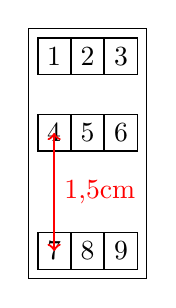
\begin{tikzpicture}
\matrix [row sep=5mm,draw,nodes=draw]
{
\node {1}; & \node {2};& \node {3}; \\
\node(a) {4} ; & \node {5}; & \node {6};\\[10mm,between origins]
\node(b) {7}; &\node {8}; & \node {9}; \\
};
\draw [<->,red,thick] (a.center) -- (b.center) node [right,midway] {1,5cm};
\end{tikzpicture}
\\ \hline 
\rouge{[1cm]} & \rouge{[1cm,between origins]}
\\ \hline 
\end{tabular} 

\bigskip

\begin{tabular}{|c|c|} \hline  
\multicolumn{2}{|c|}{\BS{matrix} [ \rouge{column sep=5mm},draw,nodes=draw]} \\
\multicolumn{2}{|c|}{ \{ \BS{node} \AC{1}; \& \BS{node} \AC{2}; \& \BS{node} \AC{3}; \BS{}\BS{}  } \\
\multicolumn{2}{|c|}{ \BS{node} \AC{4} ; \& \BS{node}  \AC{5}; \& \rouge{[1cm]}\BS{node}  \AC{6};  \BS{}\BS{}  } \\
\multicolumn{2}{|c|}{ \BS{node} \AC{7}; \& \BS{node}\AC{8}; \& \BS{node}\AC{9}; \BS{}\BS{} \}  } 
\\ \hline  

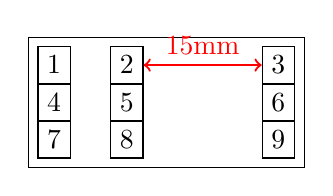
\begin{tikzpicture}
\matrix [draw,nodes=draw,column sep=5mm]
{
\node {1}; & \node(a) {2}; &[1cm] \node(b) {3}; \\
\node {4}; & \node{5}; & \node {6}; \\
\node {7}; & \node{8}; & \node {9}; \\
};
\draw [<->,red,thick] (a.east) -- (b.west) node [above,midway] {15mm};
\end{tikzpicture}
&  
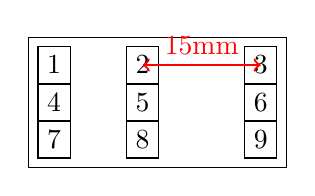
\begin{tikzpicture}
\matrix [draw,nodes=draw,column sep=5mm]
{
\node {1}; &[2mm] \node(a){2}; &[1cm,between origins] \node(b){3}; \\
\node {4}; & \node {5}; & \node {6}; \\
\node {7}; & \node {8}; & \node {9}; \\
};
\draw [<->,red,thick] (a.center) -- (b.center) node [above,midway] {15mm};
\end{tikzpicture}
\\ \hline  
\rouge{[1cm]}
&  
\rouge{[1cm,between origins]}
\\ \hline 
\end{tabular} 




\bigskip

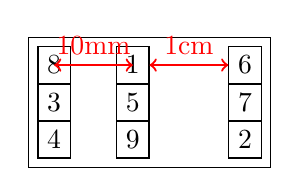
\begin{tikzpicture}
\matrix [draw,nodes=draw,column sep={1cm,between origins}]
{
\node (a) {8}; & \node (b) {1}; &[between borders] \node (c) {6}; \\
\node {3}; & \node {5}; & \node {7}; \\
\node {4}; & \node {9}; & \node {2}; \\
};
\draw [<->,red,thick] (a.center) -- (b.center) node [above,midway] {10mm};
\draw [<->,red,thick] (b.east) -- (c.west) node [above,midway] {1cm};
\end{tikzpicture}



\SbSbSSCT{Format des cellules}{Cell Styles and Options}

\noindent 

\begin{tabular}{|c|} \hline  
\BS{matrix} [nodes=draw,nodes=\AC{\rouge{fill}=blue!10\rouge{,minimum size}=1cm}]
\\ \hline  
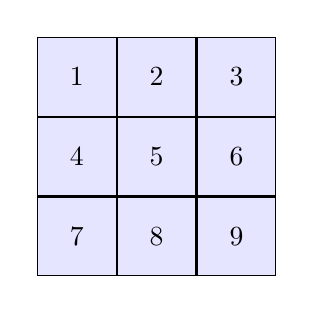
\begin{tikzpicture}
\matrix [nodes=draw,nodes={fill=blue!10,minimum size=1cm}]
{
\node {1}; & \node{2}; & \node {3}; \\
\node {4}; & \node{5}; & \node {6}; \\
\node {7}; & \node{8}; & \node {9}; \\
};
\end{tikzpicture}
\\ \hline 
\end{tabular} 


\bigskip 


\begin{tabular}{|c|c|c|} \hline 
\multicolumn{3}{|c|}{\BS{matrix}[\rouge{row 2/.style}=\AC{red}]}
 \\ \hline 
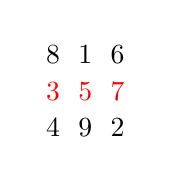
\begin{tikzpicture}
\matrix[row 2/.style={red}]
{
\node {8}; & \node{1}; & \node {6}; \\
\node {3}; & \node{5}; & \node {7}; \\
\node {4}; & \node{9}; & \node {2}; \\
};
\end{tikzpicture}
&  
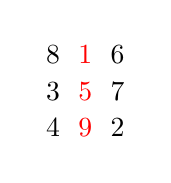
\begin{tikzpicture}
\matrix[column 2/.style={red}]
{
\node {8}; & \node{1}; & \node {6}; \\
\node {3}; & \node{5}; & \node {7}; \\
\node {4}; & \node{9}; & \node {2}; \\
};
\end{tikzpicture}
&  
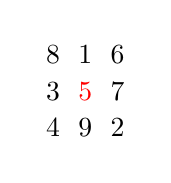
\begin{tikzpicture}
\matrix[row 2 column 2/.style={red}]
{
\node {8}; & \node{1}; & \node {6}; \\
\node {3}; & \node{5}; & \node {7}; \\
\node {4}; & \node{9}; & \node {2}; \\
};
\end{tikzpicture}
\\ \hline 
row 2/.style=\AC{red} & column 2/.style=\AC{red}  & row 2 column 2/.style=\AC{red}\\ 
\hline 
\end{tabular} 

\bigskip 

\begin{tabular}{|c|c|c|} \hline 
\multicolumn{3}{|c|}{\BS{matrix}[column 1/.style=\AC{anchor=west}]}
 \\ \hline 
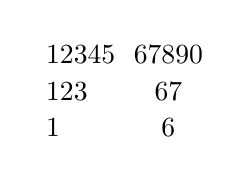
\begin{tikzpicture}
\matrix[column 1/.style={anchor=west}]
{
\node {12345};  & \node {67890}; \\
\node {123}; & \node{67};  \\
\node {1}; & \node{6}; & \\
};
\end{tikzpicture}
&  
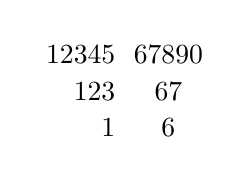
\begin{tikzpicture}
\matrix[column 1/.style={anchor=east}]
{
\node {12345};  & \node {67890}; \\
\node {123}; & \node{67};  \\
\node {1}; & \node{6}; & \\
};
\end{tikzpicture}
&  
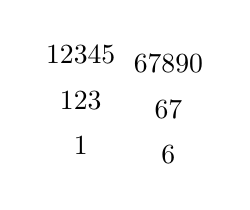
\begin{tikzpicture}
\matrix[column 1/.style={anchor=base}]
{
\node {12345};  & \node {67890}; \\
\node {123}; & \node{67};  \\
\node {1}; & \node{6}; & \\
};
\end{tikzpicture}
\\  \hline  
[\rouge{column 1/.style}={anchor=west}]& [\rouge{column 1/.style}={anchor=east}] & [\rouge{column 1/.style}={anchor=base}]\\ 
\hline 
\end{tabular} 

\bigskip

\begin{tabular}{|c|c|c|c|} \hline
\multicolumn{4}{|c|}{\BS{matrix}[matrix of nodes,\RDD{every odd column}/.style={red}]}
 \\ \hline 
\begin{tikzpicture}
\matrix [matrix of nodes,every odd column/.style={red}]
{
a & b & c & d \\
e & f & g & h \\
i & j & k & l \\
};
\end{tikzpicture}
&  
\begin{tikzpicture}
\matrix [matrix of nodes,every even column/.style={red}]
{
a & b & c & d \\
e & f & g & h \\
i & j & k & l \\
};
\end{tikzpicture}
&  
\begin{tikzpicture}
\matrix [matrix of nodes,every odd row/.style={red}]
{
a & b & c & d \\
e & f & g & h \\
i & j & k & l \\
};
\end{tikzpicture}
&  
\begin{tikzpicture}
\matrix [matrix of nodes,every even row/.style={red}]
{
a & b & c & d \\
e & f & g & h \\
i & j & k & l \\
};
\end{tikzpicture}
\\ 
\hline 
\RDD{every odd column} & \RDD{every even column} & \RDD{every odd row}  & \RDD{every even row} \\ 
\hline 
\end{tabular} 


\bigskip


\begin{tabular}{|c|} \hline  
\BS{matrix} [draw,matrix of nodes,\rouge{execute at begin cell}=\AC{(}]
\\ \hline  
\begin{tikzpicture}
\matrix [draw,matrix of nodes,execute at begin cell={(}]
{
1 & 2 &   \\
4 &   & 6 \\
  &   & 9 \\
};
\end{tikzpicture}
\\ \hline 
\end{tabular} 

\bigskip

\begin{tabular}{|c|} \hline  
\BS{tikz} 
[matrix of nodes/.style=\AC{
execute at begin cell=\BS{node}\BS{bgroup} , \\
\rouge{execute at end cell}=\$m\wedge 2\$\BS{egroup}; 
}] \\
\BS{matrix} [draw,matrix of nodes
]
\\ \hline  
\tikz 
[matrix of nodes/.style={
execute at begin cell=\node\bgroup ,
execute at end cell=$m^2$\egroup;
}]
\matrix [draw,matrix of nodes
]
{1 & 2 &  \\
4 &   & 6 \\
  & 8 & 9 \\
};
\\ \hline 
\end{tabular}

\bigskip

\begin{tabular}{|c|} \hline 

 \BS{matrix} [raw,matrix of nodes, \rouge {execute at empty cell}=\BS{node}\AC{- -}; ]
\\ \hline 
 
\begin{tikzpicture}
\matrix [draw,matrix of nodes,execute at empty cell=\node{--};]
{
1 & 2 & \\
4 & & 6 \\
& & 9 \\
};
\end{tikzpicture}
\\ \hline  
\end{tabular} 


\newpage
\SbSbSSCT{Points d'ancrage}{Anchoring a Matrix}

\begin{center}
\RRR{20-4}
\end{center}

\begin{tabular}{|c|c|c|} \hline 
\multicolumn{3}{|c|}{
\BS{matrix} [draw=red,nodes=draw,\RDD{matrix anchor}=east](XXX) at (1,1) }
\\ \hline  
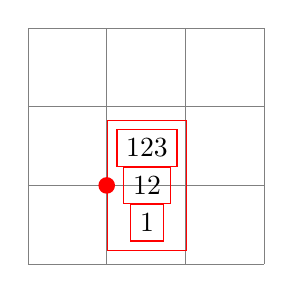
\begin{tikzpicture}
\draw[help lines] (0,0) grid (3,3);
\matrix [draw=red,nodes=draw,matrix anchor=west](XXX) at (1,1)
{
\node {123}; \\ 
\node {12}; \\
\node {1}; \\
};
\fill[red](XXX.west) circle (3pt);
\end{tikzpicture}
&  
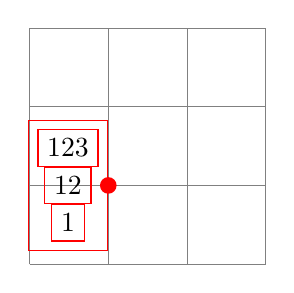
\begin{tikzpicture}
\draw[help lines] (0,0) grid (3,3);
\matrix [draw=red,nodes=draw,matrix anchor=east](XXX) at (1,1)
{
\node {123}; \\ 
\node {12}; \\
\node {1}; \\
};
\fill[red] (XXX.east) circle (3pt);
\end{tikzpicture}
&  
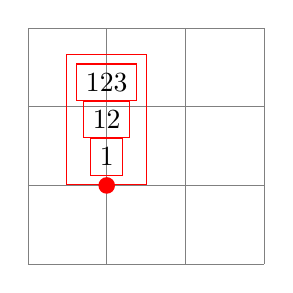
\begin{tikzpicture}
\draw[help lines] (0,0) grid (3,3);
\matrix [draw=red,nodes=draw,matrix anchor=south](XXX) at (1,1)
{
\node {123}; \\ 
\node {12}; \\
\node {1}; \\
};
\fill[red](XXX.south) circle (3pt);
\end{tikzpicture}

\\  \hline 
matrix anchor=west & matrix anchor=east & matrix anchor=south 
\\ \hline 
\end{tabular} 

\bigskip 
\begin{tabular}{|c|c|c|c|} \hline 
\multicolumn{2}{|c|}{\BS{matrix} [draw=red,nodes=draw,\rouge{anchor=west}] }
\\ \hline  
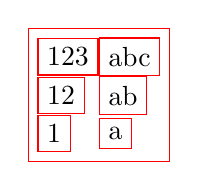
\begin{tikzpicture}
\matrix [draw=red,nodes=draw,anchor=west] 
{
\node {123}; & \node {abc}; \\ 
\node {12}; & \node {ab}; \\
\node {1}; & \node {a}; \\
};
\end{tikzpicture}
&  
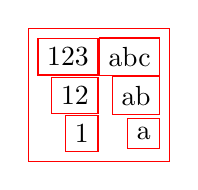
\begin{tikzpicture}
\matrix [draw=red,nodes=draw,anchor=east] 
{
\node {123};& \node {abc}; \\ 
\node {12};  &\node {ab};\\
\node {1};  & \node {a}; \\
};
\end{tikzpicture}

\\ \hline  
anchor=west & anchor=east  \\ 
\hline 
\end{tabular} 

\bigskip 


\begin{tabular}{|c|c|}\hline  
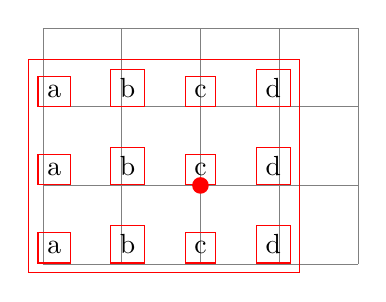
\begin{tikzpicture}[baseline=1cm]
\draw[help lines] (0,0) grid (4,3);
\matrix[draw=red,nodes=draw ,matrix anchor=inner node.south,anchor=base, row sep=5mm, column sep=5mm] at (2,1)
{
\node {a}; & \node {b}; & \node {c}; & \node {d}; \\
\node {a}; & \node {b}; & \node(inner node){c}; & \node {d}; \\
\node {a}; & \node {b}; & \node {c}; & \node {d}; \\
};
\fill[red] (inner node.south) circle (3pt);
\end{tikzpicture}
&  
\parbox{10.5cm}{
\BS{matrix}[draw=red,nodes=draw, \\ 
\RDD{ matrix anchor}=\blll{inner node}.south, anchor=base, \\
  row sep=5mm,column sep=5mm] at (2,1) \\
\{ \\
\BS{node} \AC{a}; \& \BS{node} \AC{b}; \& \BS{node} \AC{c}; \& \BS{node} \AC{d};  \BS{}\BS{} \\
\BS{node} \AC{a}; \& \BS{node} \AC{b}; \& \BS{node}(\blll{inner node})\AC{c}; \& \BS{node} \AC{d};  \BS{}\BS{} \\
\BS{node}\AC{a}; \& \BS{node} \AC{b}; \& \BS{node}\AC{c}; \& \BS{node} \AC{d}; \BS{}\BS{}  \\
\};
}
\\ \hline 
\end{tabular} 


\SbSbSSCT{Changement du séparateur}{Considerations Concerning Active Characters}

\begin{center}
\RRR{20-5}
\end{center}

\begin{tabular}{|c|c|} \hline  
\tikz[baseline=0pt]
\matrix [ampersand replacement=\|]
{
\draw (0,0) circle (4mm); \| \node[rotate=10] {Hello}; \\
\draw (0.2,0) circle (2mm); \| \fill[red] (0,0) circle (3mm); \\
};
& 
\parbox{12cm}{ 
\BS{tikz}
\BS{matrix} [\RDD{ampersand replacement}=\blll{\BS{|}} ] \\
\{ \\
\BS{draw} (0,0) circle (4mm); \blll{\BS{|} }  \BS{node}[rotate=10] \AC{Hello}; \BS{}\BS{} \\
\BS{draw} (0.2,0) circle (2mm);  \blll{\BS{|} }   \BS{fill}[red] (0,0) circle (3mm); \BS{}\BS{} \\
\}; \\
}
\\ \hline 
\end{tabular} 


\SbSSCT{Matrice de n\oe uds (compléments) }{Matrix Library}

 \maboite{\BS{usetikzlibrary}\AC{matrix}}
\label{lib-matrix}


\begin{center}
\RRR{57-1}
\end{center}

\begin{tabular}{|c|c|} \hline  
\begin{tikzpicture}[baseline=0pt]
\matrix (XXX) [matrix of nodes]
{
1 & 2 & 3 \\
4 & 5 & 6 \\
7 & 8 & 9 \\
};
\end{tikzpicture}
& 
\parbox{10cm}{ 
\BS{begin}\AC{tikzpicture} \\
\BSS{matrix}  [matrix of nodes]\\
\{ \\
1 \hspace{3mm} \& \hspace{3mm}  2 \hspace{3mm} \& \hspace{3mm} 3 \hspace{3mm} \BS{}\BS{}   \\
4 \hspace{3mm} \& \hspace{3mm}  5 \hspace{3mm} \& \hspace{3mm} 6 \hspace{3mm} \BS{}\BS{}  \\
7 \hspace{3mm} \& \hspace{3mm}  8 \hspace{3mm} \& \hspace{3mm} 9 \hspace{3mm} \BS{}\BS{} \\
\}; \\
\BS{end}\AC{tikzpicture}
}
\\ \hline  
\end{tabular} 

\bigskip

\begin{tabular}{|c|c|} \hline  
\begin{tikzpicture}[baseline=0pt]
\matrix (XXX) [matrix of nodes,column sep=.5cm,row sep=.5cm,every node/.style=draw]
{
1 & 2 & 3 \\
4 & 5 & 6 \\
7 & 8 & 9 \\
};
\draw[thick,red,->] (XXX-1-1) -- (XXX-2-3);
\end{tikzpicture}
& 
\parbox{10cm}{ 
\BS{begin}\AC{tikzpicture} \\
\BSS{matrix} \blll{(XXX)} [matrix of nodes,column sep=.5cm,row sep=.5cm,every node/.style=draw]\\
\{ \\
1 \hspace{3mm} \& \hspace{3mm} 2 \hspace{3mm} \& \hspace{3mm} 3 \hspace{3mm} \BS{}\BS{}   \\
4 \hspace{3mm} \& \hspace{3mm} 5 \hspace{3mm} \& \hspace{3mm} 6 \hspace{3mm} \BS{}\BS{}  \\
7 \hspace{3mm} \& \hspace{3mm} 8 \hspace{3mm} \& \hspace{3mm} 9 \hspace{3mm} \BS{}\BS{} \\
\}; \\
\BS{draw}[thick,red,->] \blll{(XXX-1-1)} - - \blll{(XXX-2-3)} ; \\
\BS{end}\AC{tikzpicture}
}
\\ \hline  
\end{tabular} 

\bigskip


\begin{tabular}{|c|c|} \hline  
\begin{tikzpicture}
\matrix [matrix of nodes,column sep=.5cm,row sep=.5cm,every node/.style=draw]
{
8 & 1 & 6 \\
3 & 5 & |[red]| 7 \\
4 & 9 & 2 \\
};
\end{tikzpicture}
&  
\begin{tikzpicture}
\matrix [matrix of nodes]
{
1 & \& &  2 & \& &  3 				& \BS{}\BS{} \\
4 & \& & 5 	& \& & \rouge{ $|[$red$]|$} 6 & \BS{}\BS{} \\
7 & \& & 8 	& \& & 9 				& \BS{}\BS{} \\
};
\end{tikzpicture}
\\ \hline 
\end{tabular}  


\bigskip

\begin{tabular}{|c|c|} \hline 
\begin{tikzpicture}[baseline=-1cm] 
\matrix [matrix of nodes,column sep=.5cm,row sep=.5cm,every node/.style=draw]
{
AAA 			& |[circle]| BBB \\
CCC & |(d) [isosceles triangle]| DDD \\
| [ellipse]| EEE &  FFF \\
};
\end{tikzpicture}
& 
\begin{tikzpicture}
\matrix [matrix of nodes]
{
AAA & \& & \rouge{ $|[$circle$]|$} BBB &  \BS{}\BS{} \\
CCC & \& &\rouge{ $|[$isosceles triangle$]|$} DDD 	&  \BS{}\BS{} \\
\rouge{ $|[$ellipse$]|$} EEE & \& & FFF & \BS{}\BS{} \\
};
\end{tikzpicture}
\\ \hline 
\end{tabular} 


\bigskip

\begin{tabular}{|c|c|} \hline 
\begin{tikzpicture}[baseline=-2cm] 
\matrix [matrix of nodes,column sep=.5cm,row sep=.5cm,every node/.style=draw]
{
|(a)| AAA 	& |(b)| BBB \\
|(c)| CCC 	& |(d)| DDD \\
|(e)| EEE 	& |(f)| FFF \\
};
\draw (a) -- (d);
\draw (d) -- (f);
\end{tikzpicture}
&  
\begin{tikzpicture}
\node at (0,1.5) [text width=10cm]
{\BS{matrix} [matrix of nodes,column sep=.5cm,row sep=.5cm,every node/.style=draw] \\
\{ 
};
\matrix [matrix of nodes]
{
\rouge{ $|$(a)$|$} AAA & \& & \rouge{ $|$(b)$|$} BBB &  \BS{}\BS{} \\
\rouge{ $|$(c)$|$} CCC & \& & \rouge{ $|$(d)$|$} DDD 	&  \BS{}\BS{} \\
\rouge{ $|$(e)$|$} EEE & \& & \rouge{ $|$(f)$|$} FFF & \BS{}\BS{} \\
};

\node at (0,-1.2) [text width=10cm]
{  \}; \\ 
\BS{draw} (a) - - (d); \\ \BS{draw} (d) - - (f);
};
\end{tikzpicture}
\\ \hline 
\end{tabular} 

\bigskip


\begin{tabular}{|c|c|} \hline  
\begin{tikzpicture}
\matrix [matrix of nodes]
{
1 &[1cm] 2 &[5mm] |[red]| 3 \\
4 & 5 &  6 \\
7 & 8 & 9 \\
};
\end{tikzpicture}
&
\begin{tikzpicture}
\matrix [matrix of nodes]
{
1 & \& & \rouge{\lbrack 1cm \rbrack} 2 & \& &\rouge{\lbrack 5mm \rbrack} |[red]| 3 & \BS{}\BS{} \\
4 & \& & 5 & \& & 6 & \BS{}\BS{} \\
7 & \& & 8 & \& & 9 & \BS{}\BS{} \\
};
\end{tikzpicture}

\\ \hline 
\end{tabular} 



\bigskip

\begin{tabular}{|c|c|} \hline  
\begin{tikzpicture}[baseline=0pt]
\matrix [matrix of math nodes]
{
A_1 & A_2 & A_3 \\
a_4 & a_5 &  a_6 \\
a^7 & a^8 & a^9 \\
};
\end{tikzpicture}
&  
\parbox{8cm}{ 
\BSS{matrix}  [\rouge{ matrix of math nodes}]\\
\{ \\
A\_1 \hspace{2mm}  \& \hspace{2mm}  A\_2 \hspace{2mm}  \& \hspace{2mm}  A\_3 \hspace{2mm}   \BS{}\BS{}   \\
a\_4 \hspace{2mm}  \& \hspace{2mm}  a\_5 \hspace{2mm}  \&  \hspace{2mm}  a\_6 \hspace{2mm}  \BS{}\BS{}  \\
a\land 7 \hspace{2mm}  \& \hspace{2mm}  a\land 8 \hspace{2mm}  \& \hspace{2mm}  a\land 9 \hspace{2mm}   \BS{}\BS{} \\
\}; 
}
\\ \hline  
\end{tabular} 

\bigskip

\begin{tabular}{|c|c|} \hline  
\begin{tikzpicture}[baseline=0pt]
\matrix [matrix of math nodes,nodes={circle,draw}]
{
a_1 & & a_3 \\
a_4 & & a_6 \\
a_7 & a_8 & \\
};
\end{tikzpicture}
&  
\parbox{10cm}{ 
\BSS{matrix}  [matrix of math nodes,\rouge{nodes={circle,draw}}]\\
\{ \\
A\_1 \hspace{2mm}  \& \hspace{12mm}  \& \hspace{2mm}  A\_3 \hspace{2mm}   \BS{}\BS{}   \\
a\_4 \hspace{2mm}  \& \hspace{12mm}  \& \hspace{2mm}   a\_6 \hspace{2mm}  \BS{}\BS{}  \\
a\_ 7 \hspace{2mm}  \& \hspace{2mm}  a\_ 8 \hspace{2mm}  \& \hspace{12mm}    \BS{}\BS{} \\
\}; 
}
\\ \hline 
\end{tabular} 

\bigskip

\begin{tabular}{|c|c|} \hline  
\begin{tikzpicture}[baseline=0pt]
\matrix [matrix of math nodes,nodes={circle,draw},nodes in empty cells]
{
a_1 & & a_3 \\
a_4 & & a_6 \\
a_7 & a_8 & \\
};
\end{tikzpicture}
&  
\parbox{10cm}{ 
\BSS{matrix}  [matrix of math nodes,nodes={circle,draw} ,\rouge{nodes in empty cells}]\\
\{ \\
A\_1 \hspace{2mm}  \& \hspace{12mm}  \& \hspace{2mm}  A\_3 \hspace{2mm}   \BS{}\BS{}   \\
a\_4 \hspace{2mm}  \& \hspace{12mm}  \& \hspace{2mm}   a\_6 \hspace{2mm}  \BS{}\BS{}  \\
a\_ 7 \hspace{2mm}  \& \hspace{2mm}  a\_ 8 \hspace{2mm}  \& \hspace{12mm}    \BS{}\BS{} \\
\}; 
}
\\ \hline 
\end{tabular} 

\SbSbSSCT{Texte dans les n\oe uds}{Characters in Matrices of Nodes}

\begin{center}
\RRR{57-2}
\end{center}


\begin{tabular}{|c|c|} \hline  
\begin{tikzpicture}[baseline=0pt]
\matrix [matrix of nodes,nodes={text width=2cm,draw}]
{
aaa  & bbb \\ 
ccc \\
eee & fff\\
};
\end{tikzpicture}
&  
\parbox{10cm}{ 
\BSS{matrix}  [matrix of nodes,\rouge{nodes=\AC{text width=2cm,draw}} ]\\
\{ \\
aaa \&  bbb \BS{}\BS{}  \\
ccc \BS{}\BS{}  \\
eee \& fff \BS{}\BS{}  \\
\}; 
}
\\ \hline 
\end{tabular} 

\bigskip

\begin{tabular}{|c|c|}  \hline  
\begin{tikzpicture}[baseline=0cm]
\matrix [matrix of nodes,nodes={text width=2cm,draw}]
{
1 & {aaa \\ bbb \\ ccc } \\
2 & ddd \\
};
\end{tikzpicture}
&  
\parbox{10cm}{ 
\BSS{matrix}  [matrix of nodes,nodes=\AC{text width=2cm,draw} ]\\
\{ \\
1 \& \& \rouge { \AC{aaa \BS{}\BS{} bbb \BS{}\BS{} ccc } } \BS{}\BS{}   \\
2 \& \& ddd \BS{}\BS{}  \\
\}; 
}
\\ \hline 
\end{tabular} 

\bigskip

\SbSbSSCT{Délimiteurs}{Delimiters}


\begin{center}
\RRR{57-3}
\end{center}

\bigskip

\begin{tabular}{|c|c|c|c|} \hline 
\multicolumn{4}{|c|}{\BS{matrix} [matrix of math nodes,\RDD{left delimiter}=( ]}
\\ \hline  
\begin{tikzpicture}
\matrix [matrix of math nodes,left delimiter=( ]
{
a_1 & a_2 & a_3 \\
a_4 & a_5 & a_6 \\
a_7 & a_8 & a_9 \\
};
\end{tikzpicture}
&  
\begin{tikzpicture}
\matrix [matrix of math nodes,right delimiter=\}]
{
a_1 & a_2 & a_3 \\
a_4 & a_5 & a_6 \\
a_7 & a_8 & a_9 \\
};
\end{tikzpicture}
&
\begin{tikzpicture}
\matrix [matrix of math nodes,above delimiter=\| ]
{
a_1 & a_2 & a_3 \\
a_4 & a_5 & a_6 \\
a_7 & a_8 & a_9 \\
};
\end{tikzpicture}
&
\begin{tikzpicture}
\matrix [matrix of math nodes,below delimiter=\rmoustache ]
{
a_1 & a_2 & a_3 \\
a_4 & a_5 & a_6 \\
a_7 & a_8 & a_9 \\
};
\end{tikzpicture}


\\  \hline 
\RDD{left delimiter}=(  & \RDD{right delimiter}=\BS{\}} & \RDD{above delimiter}=\BS{|} & \RDD{below delimiter}=\BS{rmoustache}
\\  \hline
\end{tabular} 

\bigskip
\begin{tabular}{|c|} \hline  
\BS{tikz}
\BS{node} [fill=red!20,text width=2cm,\rouge{left delimiter}=\BS{\{} ] \\
\AC{Ceci est une démonstration d'un texte  sur une largeur de 2cm.};
\\ \hline  
\tikz
\node [fill=red!20,text width=2cm,left delimiter=\{]
{Ceci est une démonstration d'un texte  sur une largeur de 2cm.};
\\ \hline 
\end{tabular} 


